\documentclass[a4paper]{article} \usepackage[backend=biber, style=numeric, sorting=none]{biblatex}
\usepackage[a4paper, left=1cm, right=1cm, top=1cm, bottom=1cm, landscape]{geometry}
% \usepackage{showframe}
\usepackage{multicol}
\usepackage{blindtext}
\usepackage{listings}
\usepackage{graphicx}
\usepackage{enumitem}
\graphicspath{{images/cs2100/}}

\begin{document}
\setlength\parindent{0pt} %TODO this somehow messes up paragraph vertical spacing as well?
\scriptsize
% \tiny
\pagenumbering{gobble}

\begin{center}
{\large CS2100 Cheatsheet 2017}\\{by vig}
\end{center}
    \begin{multicols*}{4}

% NUMBER SYSTEMS & DATA REPRESENTATION %
{\small\textbf{Number Systems \& Data Representation }}
\textbf{Sizes of data/types}
\begin{itemize}[leftmargin=*]
\itemsep -0.5em
\item byte : 8 bits \item nibble : 4 bits (half-word)
\item word : multiple bytes (1, 2, 4) (for MIPS it's 4)
\item \texttt{int} : 4 bytes (1 bit for sign, 31 for magnitude)
\item \texttt{float} : 4 bytes
\item \texttt{double} : 8 bytes
\item \texttt{char} : 1 byte
\end{itemize}

\textbf{Representation \& Complements}
\begin{itemize}[leftmargin=*]
\itemsep -0.5em
\item Convert decimal whole numbers to base $R$ : divide by R, first remainder is LSB, last is MSB
\item Convert decimal fractions to base R : multiply by R, first carry is MSB, last is LSB
\item base ${R}$ to base ${R^N}$: partition in groups of $N$ e.g groups of 4 for base 2 to base 16
\item Convert to R-1s complement : Flip the digits; \texttt{digit = R - digit}
\item Convert to Rs complement : Flip the digits, then add 1 to the number
\item 1s complement has +ive and -ive 0
\item 2s complement has only 1 representation of 0
\item 2s complement can represent an \i{additional} negative number e.g for binary, 1000 represents -8 (+8 cannot be represented in a signed 4 bit number)
\item Convert to excess X: Take number minus X (0 refers to -x)
\item IEEE 754 Floating-Point Representation:  $sign  | exponent  |  mantissa$
\item Single-precision float has 1 bit sign, 8 bit excess-127 exponent, 23 bit mantissa (normalized with a leading bit 1 i.e the mantissa is the X in 1.X)
\item Double has 1 bit sign, 11 bit excess-1023 exponent, 52 bit mantissa 
\end{itemize}

\textbf{Operations with binary numbers}
\begin{itemize}[leftmargin=*]
\itemsep -0.5em
\item 2s complement addition: Simply add \& ignore carry out of MSB
\item 2s complement subtraction: take 2s complement of number to be subtracted, then do 2s addition.
\item 1s complement addition: Add; If there is a carry out, add 1 to the result
\item 1s complement subtraction: take 1s complement of number to be subtracted, then do 1s addition.
\item check for \bf{overflow}: If result is opposite sign of both operands (that have the same sign)
\end{itemize}

% MIPS %
{\small\textbf{MIPS}}

\textbf{R, I, J format}
\begin{itemize}[leftmargin=*]
\itemsep -0.5em
\item $\bf{R}$: $Opcode, rs, rt, rd, shamt, funct$
\item $\bf{I}$: $Opcode, rs, rt, Imm$
\item rd is not used, check datasheet for instruction syntax
\item For branch, $Imm$ is the relative number of \i{words} to go to (with respect to $PC + 4$), in Sign and Magnitue representation
\item $\bf{J}$: $Opcode, Address$
\item First 4 bits are assumed to be 4 MSBs of $PC + 4$. Last 2 bits assumed to be 0 (because of word addressing)
\end{itemize}

% Instruction Set Architecture %
{\small\textbf{Instruction Set Architecture}}

\textbf{Architectures \& Endianness}
\begin{itemize}[leftmargin=*]
\itemsep -0.5em
\item Von Neumann: Data(operands) stored in memory
\item Stack: operands are on top of stack
\item Accumulator: One operator is in the accumulator (a special register)
\item Memory-memory (all operands in memory)
\item Register-Register (all operands in registers) (MIPS)
\item Big-endian: Most significant byte stored in lowest address
\item Little-endian: Least significant byte stored in lowest address (easier to read)
\end{itemize}

\textbf{Opcode encoding}
\begin{itemize}[leftmargin=*]
\itemsep -0.5em
\item To maximize, reserve 1 instruction for lesser-bit instruction types.
\item To minimize, reserve all but 1 instruction for lesser-bit instruction types
\item Forumla for maximizing: $2^{no. of bits} * (1 - F)$ where $F$ is the fraction of bits lost by reserving bits
\end{itemize}

% Boolean Algebra %
{\small\textbf{Boolean Algebra}}
\textbf{Laws}
\begin{itemize}[leftmargin=*]
\itemsep -0.5em
\item Identity: $A + 0 = A$ and $A \cdot 1 = A$
\item Complement: $A + A' = 1$ and $A \cdot A' = 0$
\item Commutative: $A + B = B + A$  and $A \cdot B = B \cdot A$
\item Associative: $A + (B + C) = (A + B) + C$ and $A \cdot (B \cdot C) = (A \cdot B) \cdot C$
\item Distributive: $A + (B \cdot C) = (A + B) \cdot (A + C)$ and $A \cdot (B + C) = (A \cdot B) + (A \cdot C)$
\item Duality (not a real law): If we flip AND/OR operators and flip the operands (0 and 1), the boolean equation still holds
\end{itemize}

\textbf{Theorems}
\begin{itemize}[leftmargin=*]
\itemsep -0.5em
\item Idempotency: $X + X = X$ and $X \cdot X = X$
\item One/Zero Element: $X + 1 = 1$ and $X \cdot 0 = 0$
\item Involution: $(X')' = X$ 
\item Absorption: \\ $X + (X \cdot Y) = X$ \\ $X \cdot (X + Y) = X$
\item Absorption (variant): \\ $X + (X' \cdot Y) = X + Y$ \\ $X \cdot (X' + Y) = X \cdot Y$
\item DeMorgans' (can be used on $>2$ variables): \\ $(X \cdot Y)' = X' + Y'$ \\ $(X + Y)' = X' \cdot Y'$
\item Concensus: \\ $(X \cdot Y) + (X' \cdot Z) + (Y \cdot Z) = (X \cdot Y) + (X' \cdot Z)$ \\ $(X + Y) \cdot (X' + Z) \cdot (Y + Z) = (X + Y) \cdot (X' + Z)$
\end{itemize}

\textbf{Minterms \& Maxterms}
\begin{itemize}[leftmargin=*]
\itemsep -0.5em
\item Sum-Of-Products (SOP): Product term or a logical sum of product terms
\item $m$interm: Product term that contains $n$ literals from all the variables
\item Product-Of-Sum (POS): Sum term or a logical product of sum terms
\item $M$axterm: Sum term that contains $n$ literals from all the variables
\item $Mx$ = $mx'$ because of De Morgan's
\item Sum of 2 distinct Maxterms is 1 e.g $M1234 + M1120 = 1$
\item Product of 2 distinct minterms is 0 e.g $m1234 \cdot m1120 = 0$
\end{itemize}

% Combinatorial Circuits %
{\small\textbf{Combinatorial Circuits}}
\\ \textbf{Gates}
\begin{itemize}[leftmargin=*]
\itemsep -0.5em
\item {AND, OR, NOT} is a complete set of logic
\item {NAND} is a complete set of logic
\item {NOR} is a complete set of logic
\item Produce SOP with $AND >> OR$ or $NAND >> NAND$
\item Produce POS with $OR >> AND$ or $NOR >> NOR$
\item With negated outputs, use NAND to simulate OR and NOR to simulate AND
\end{itemize}
{\centering 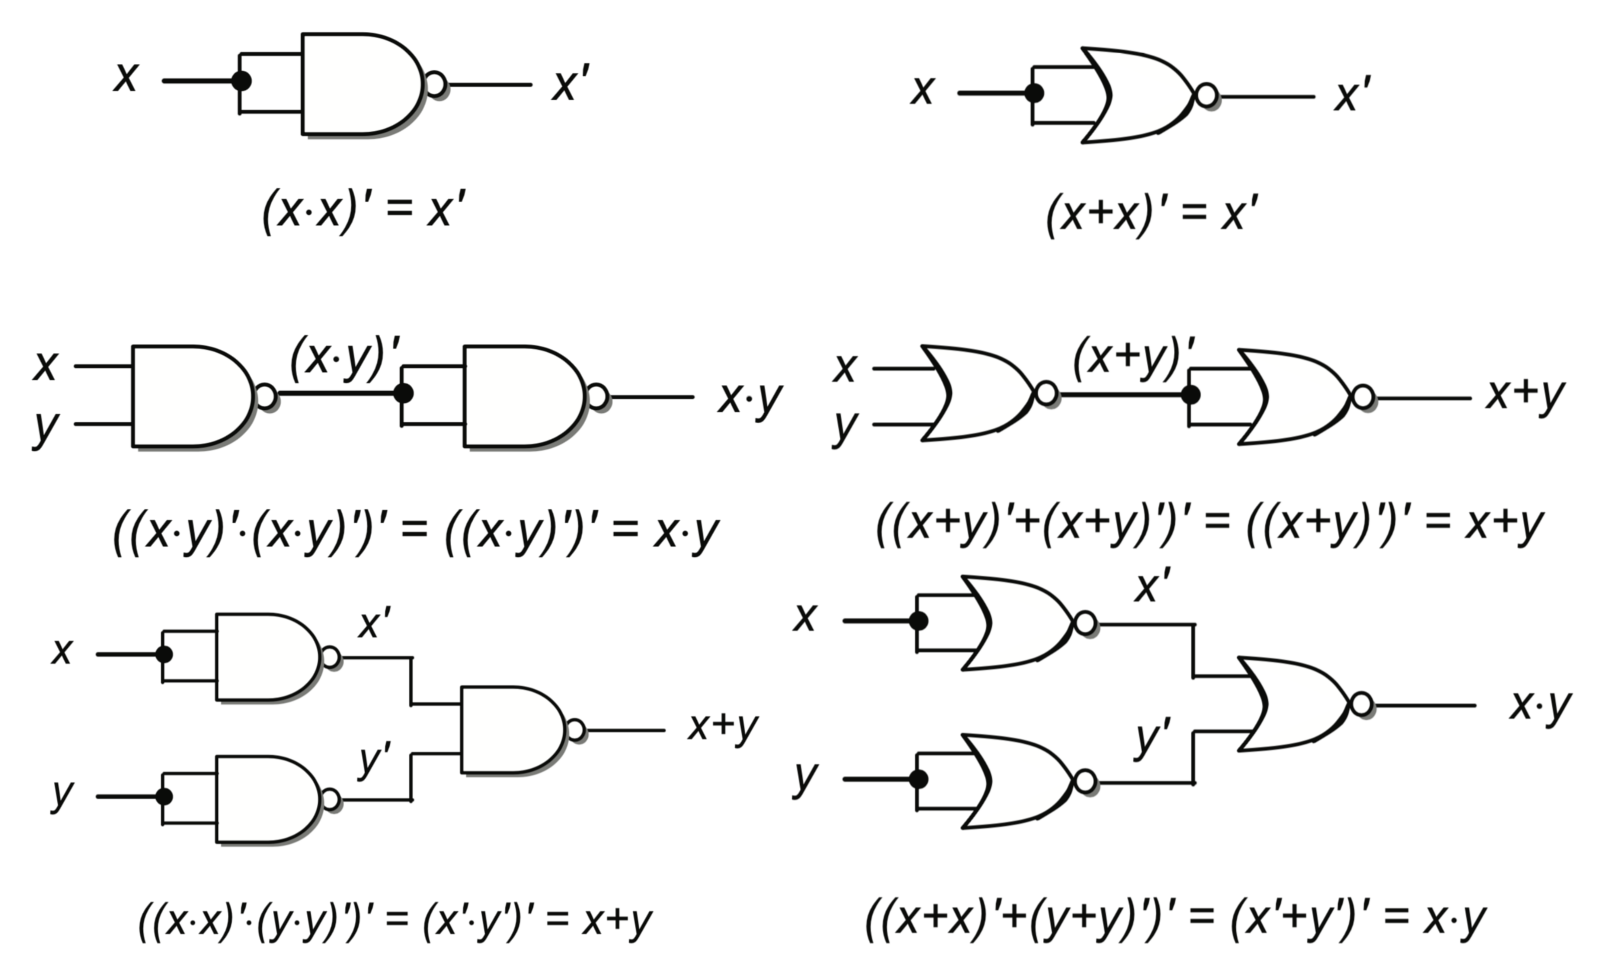
\includegraphics[scale=0.1]{nor_nand}}

\textbf{K-maps}
\begin{itemize}[leftmargin=*]
\itemsep -0.5em
\item Prime Implicant (PI) is a product term formed by combining the {\i maximum} possible no. of minterms (largest group)
\item Essential Prime Implicant (EPI) is a PI that includes at least one minterm not covered by any other group
\item Label the K-map rows/columns in a {\i gray code} manner e.g $00, 01, 11, 10$
\item Grouping $2^N$ cells(only power-sizes are allowed) eliminates n variables
\item EPIs are counted only by checking 1s, {\bf not} $X$s
\item K-maps help to obtain canonical SOP, but might not provide the simplest expression possible (need to use boolean algebra for that)
\end{itemize}

\textbf {Delays} \text{: Note that for combinatorial circuits, there is a delay: for every logic gate with $n$ inputs, calculate $delay = max(t_1, t_2, \dots t_n) + t_delay$}
{\centering 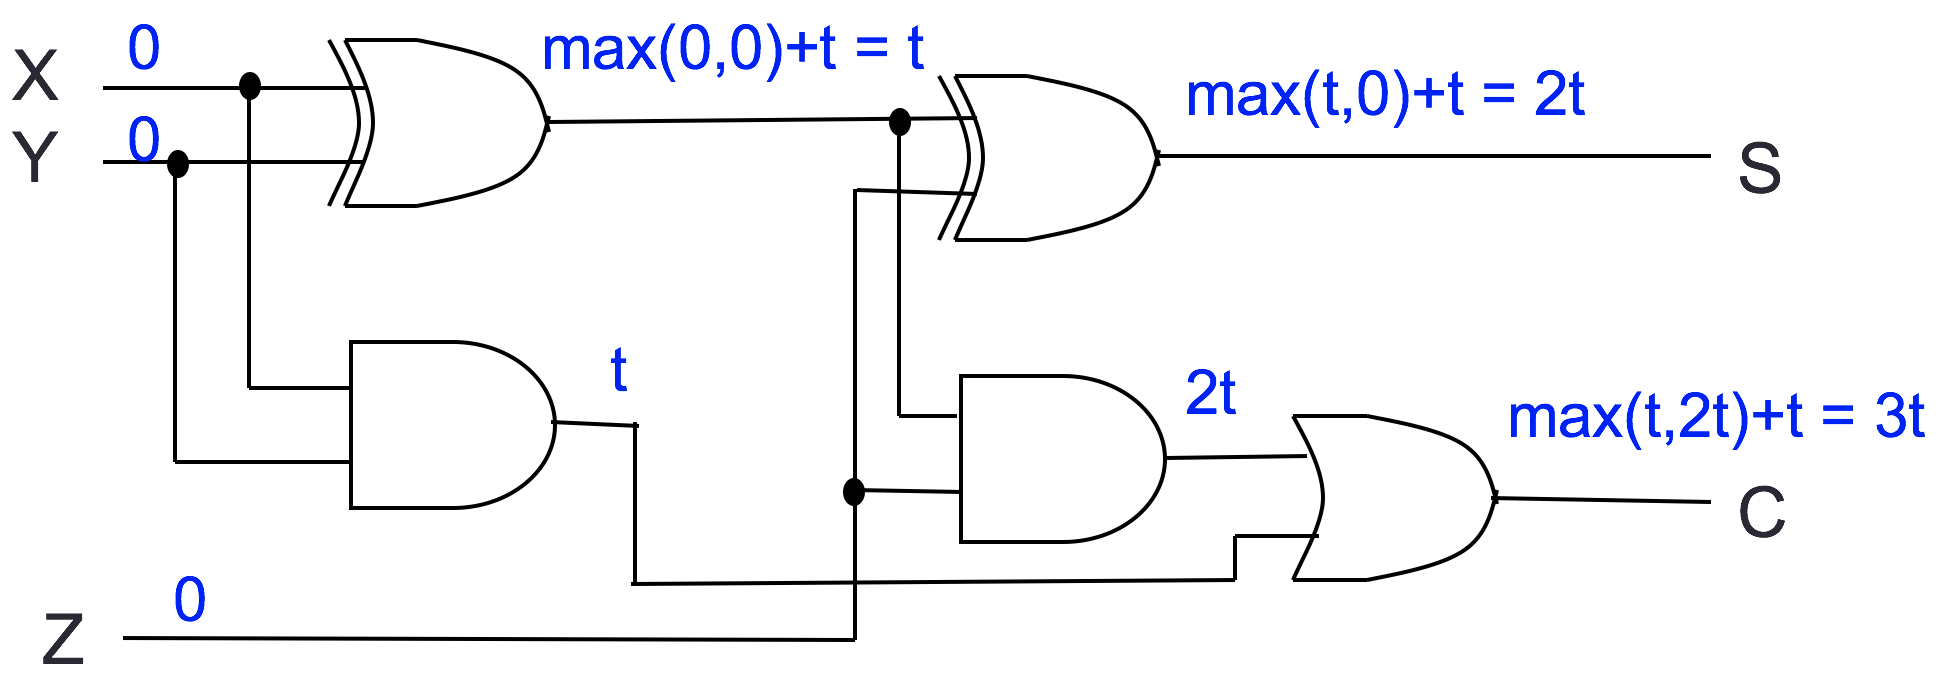
\includegraphics[scale=0.18]{circuit_delay}}


\textbf{MSI Components}
\textbf{{Decoder}}
\begin{multicols*}{2}
{\centering 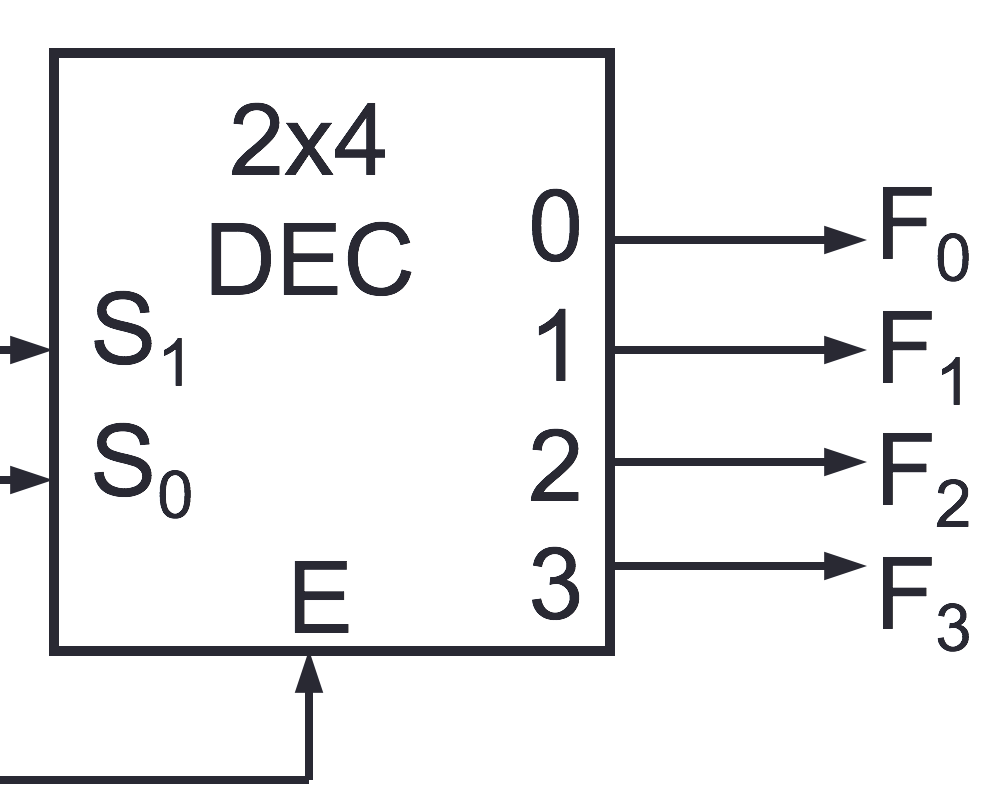
\includegraphics[scale=0.13]{decoder}}
\vfill\null
\columnbreak
Generate minterms and use OR to form a function
Alternatively, generate maxterms and use NOR
\end{multicols*}

\begin{multicols*}{2}
\textbf{{Multiplexer}}
\\ Use minterm as selection line, using 0/1 as inputs. For smaller size multiplexer, use one of the variables for input lines.
\vfill\null
\columnbreak
{\centering 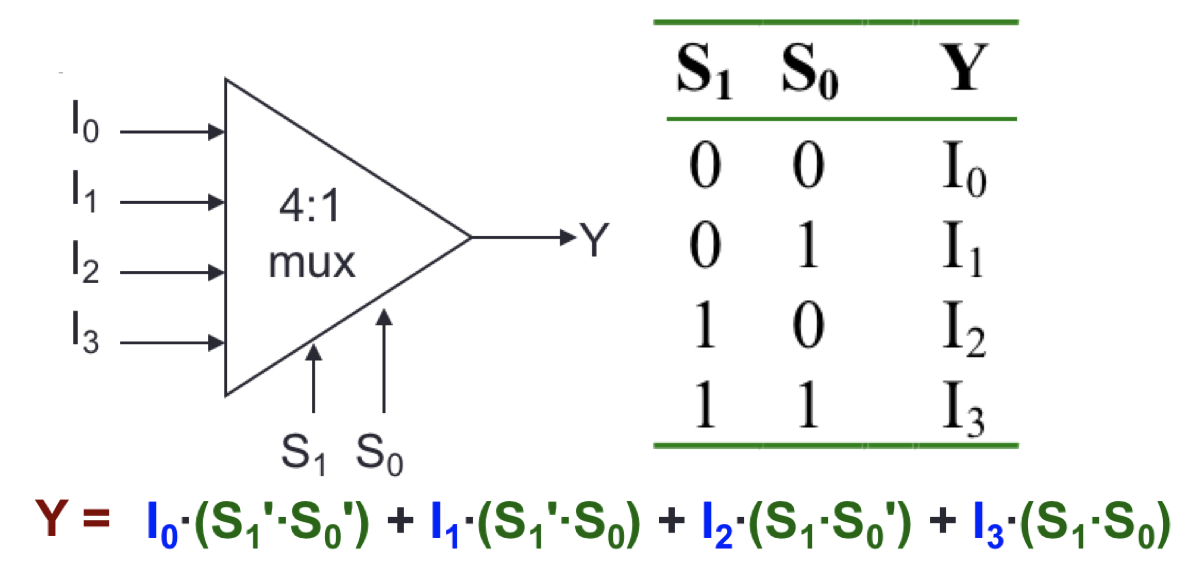
\includegraphics[scale=0.13]{multiplexer}}
\end{multicols*}

\begin{multicols*}{2}
\textbf{{Demultiplexer}}
\vfill\null
\columnbreak
{\centering 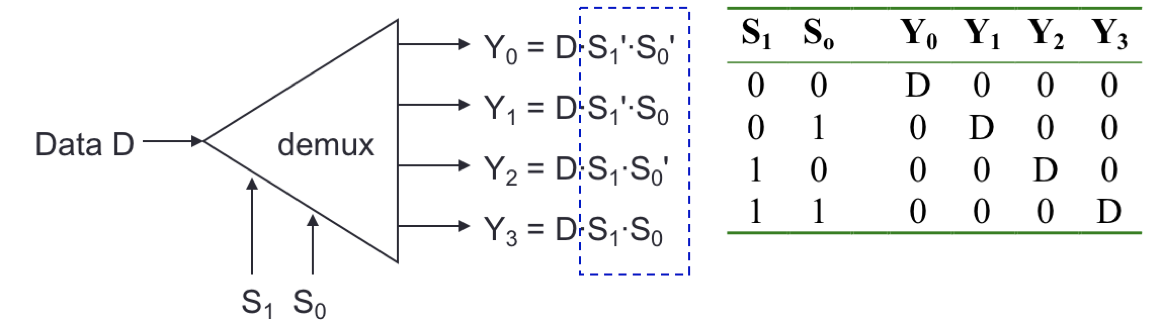
\includegraphics[scale=0.13]{demultiplexer}}
\end{multicols*}

\begin{multicols*}{2}
\textbf{{Encoder}}
\vfill\null
\columnbreak
{\centering 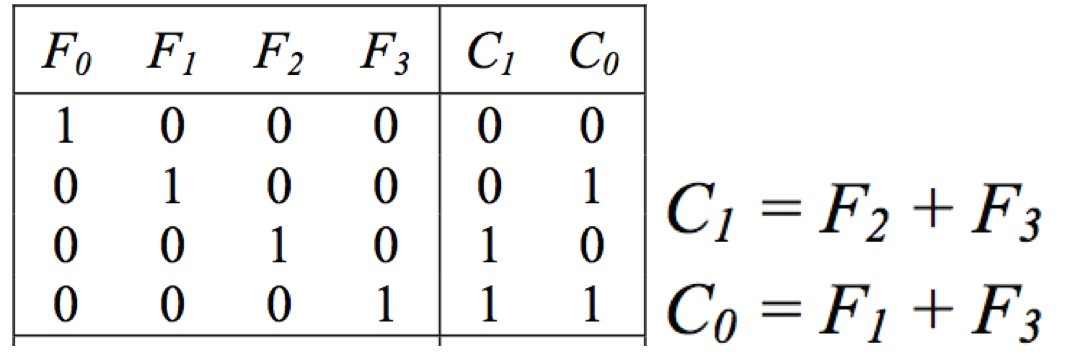
\includegraphics[scale=0.13]{encoder}}
\end{multicols*}

\begin{multicols*}{2}
\textbf{{Decoder}}
\vfill\null
\columnbreak
{\centering 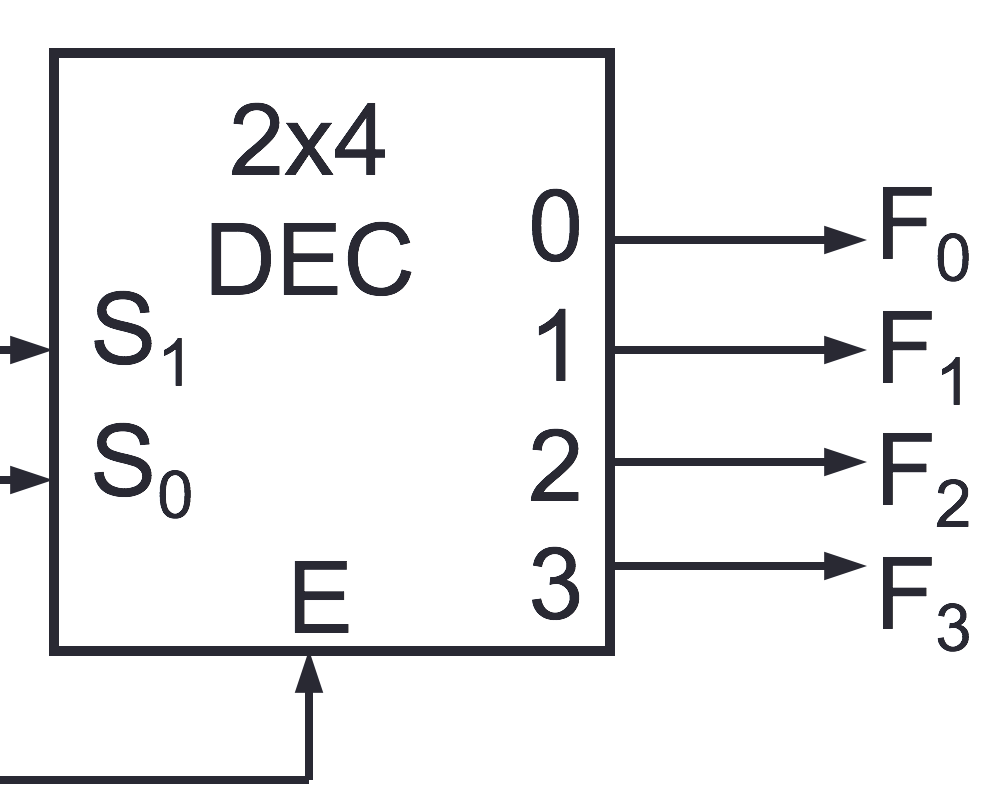
\includegraphics[scale=0.13]{decoder}}
\end{multicols*}

\begin{multicols*}{2}
\textbf{{Priority Encoder}}
\vfill\null
\columnbreak
{\centering 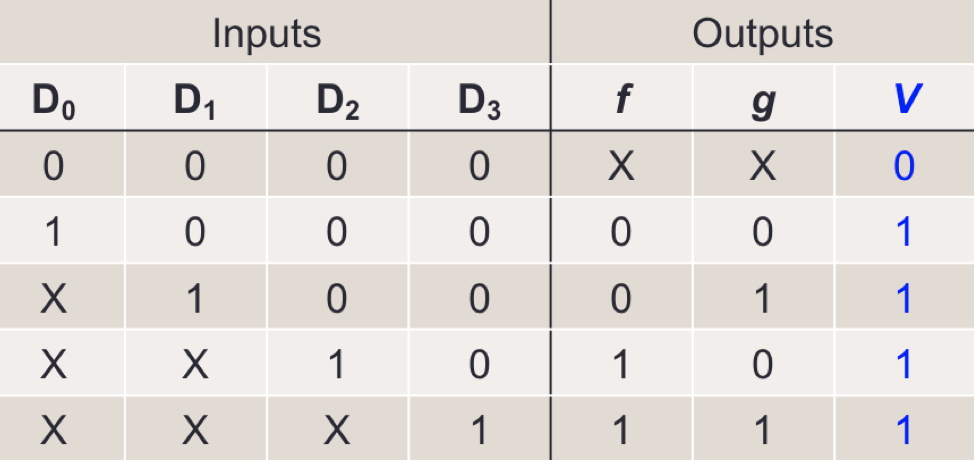
\includegraphics[scale=0.13]{priorityEncoder}}
\end{multicols*}

\begin{multicols*}{2}
\textbf{{Larger Components}}
\vfill\null
\columnbreak
{\centering 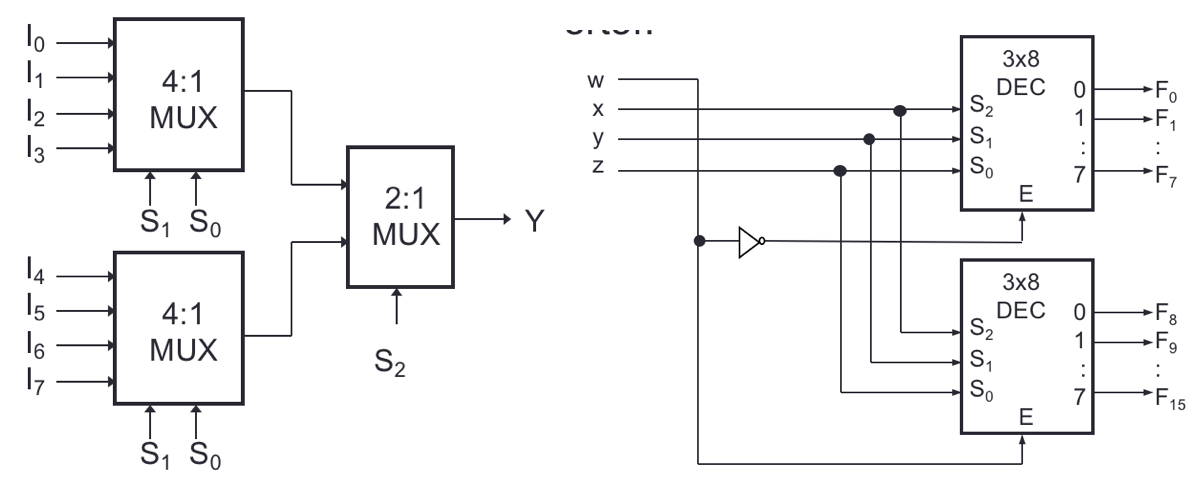
\includegraphics[scale=0.13]{largerComponents}}
\end{multicols*}

%Sequential Logic%
{\small\textbf{Sequential Logic }}
\\ \textbf{{Excitation Tables}}
\\ {\centering 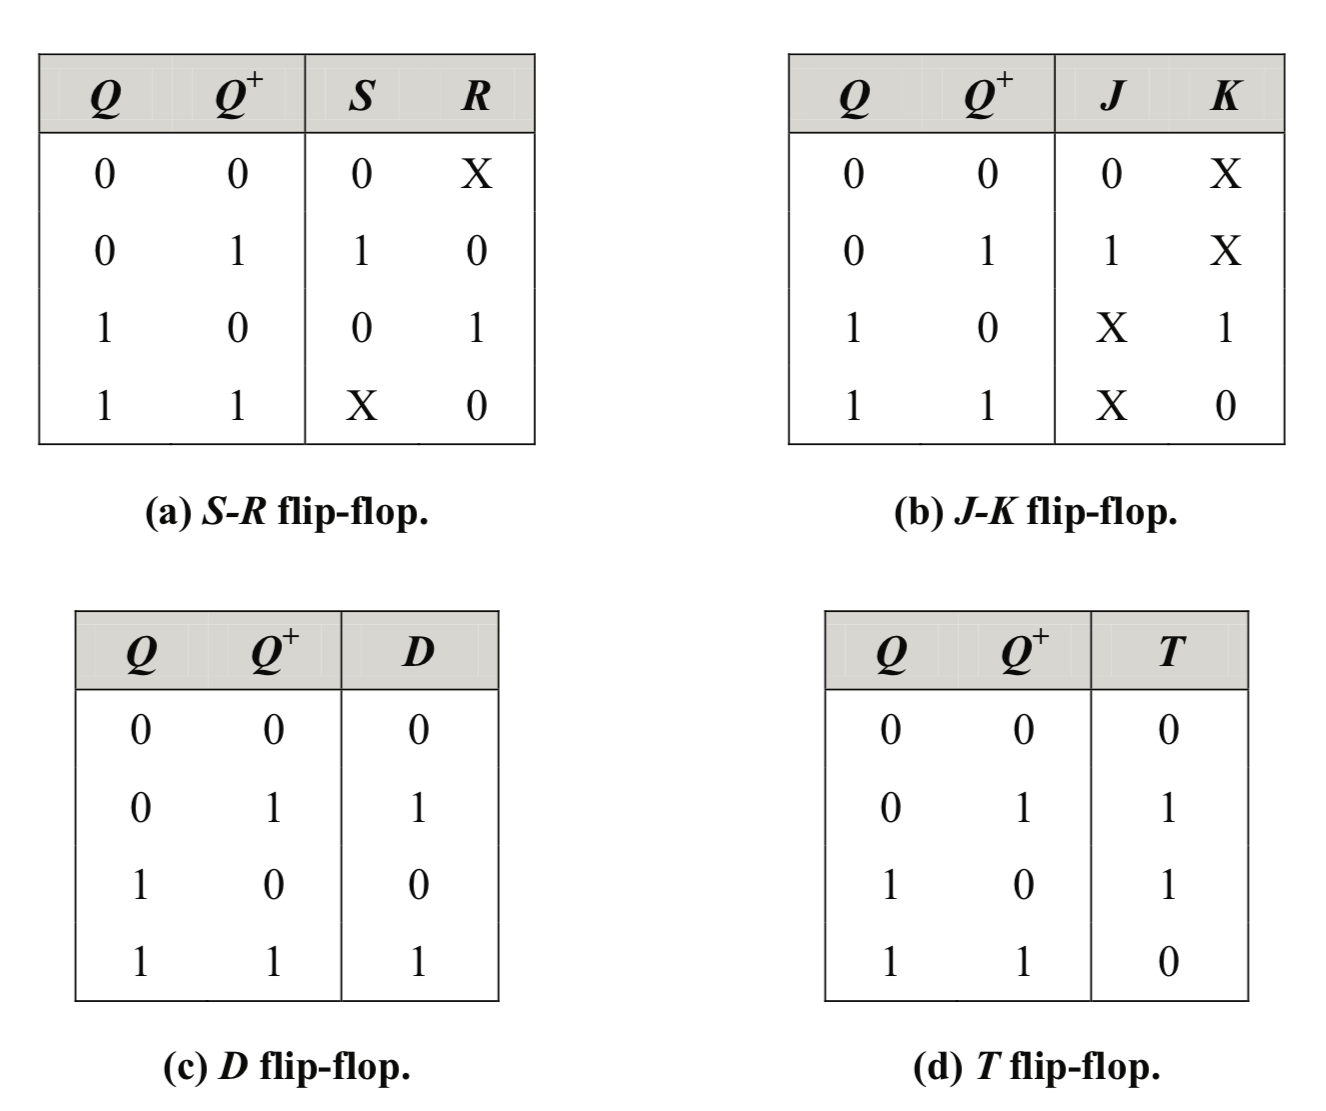
\includegraphics[scale=0.14]{excitationTables}}














% THE SUBSTITUTION MODEL %
{\small\textbf{Substitution Model}}
\begin{verbatim}
function plus_one(x) {
    return x + 1;
}

function twice(f) {
    return function(x) {
        return f(f(x));
    }
}

function n_times(f, n) {
    if (n === 1) {
        return f;
    } else {
        return function(x) {
            return f((n_times(f, n-1))(x);
        }
    }
}

function chain(f, n) {
    if (n === 1) {
        return f;
    } else {
        return (chain(f, n-1))(f);
    }
}
\end{verbatim}
\par \texttt{plus\_one(plus\_one(0))}
\par $pp(0) \rightarrow p(1) \rightarrow 2$
\\
\par \texttt{(twice(plus\_one))(0)}
\par $t(p)0 \rightarrow pp(0) \rightarrow 2$
\\
\par \texttt{(n\_times(plus\_one,4))(0)}
\par $n(p,4)(0) \rightarrow p(n(p,3))(0) \rightarrow pp(n(p,2))(0)$\\
     $\rightarrow ppp(n(p,1))(0) \rightarrow pppp(0) \rightarrow 4$
\\
\par \texttt{((n\_times(twice,3))(plus\_one))(0)}
\par $n(t,3)(p)(0) \rightarrow ttt(p)(0) \rightarrow ttpp(0) \rightarrow tpppp(0)$\\
     $\rightarrow pppppppp(0) \rightarrow p^8(0) \rightarrow 8$
\\
\par \texttt{((n\_times(chain(twice,3),2))(plus\_one))(0)}
\par $n(c(t,3),2)(p)(0) \rightarrow n(c(t,2)(t),2)(p)(0)$\\
     $\rightarrow n(c(t,1)(tt), 2)(p)(0) \rightarrow n(t(tt), 2)(p)(0)$\\
     $\rightarrow n(tttt, 2)(p)(0) \rightarrow t^8(p)(0) \rightarrow p^{2^8}(0)$\\
     $\rightarrow p^{256}(0) \rightarrow 256$
\\
\par \texttt{((chain(twice,4))(plus\_one))(0)}
\par $((c(t,4))(p))(0) \rightarrow c(t,3)(t)(p)(0) \rightarrow c(t,2)(tt)(p)(0)$\\
     $\rightarrow c(t,1)(tttt)(p)(0) \rightarrow tttttttt(p)(0) \rightarrow t^8p(0)$\\
     $\rightarrow p^{2^8}(0) \rightarrow p^{256} \rightarrow 256$
\\

% THE ENVIRONMENT MODEL %
{\small\textbf{Environment Model}}
\\ \\
To apply a function $f$,
\begin{enumerate}
\itemsep -0.5em
\item Create a new frame, $A$
\item Point $A$ back to the environment in which $f$ was defined
\item In $A$, bind the parameters of $f$ to the values of the arguments given during the function call
\item Evaluate the body of $f$ within $A$
\end{enumerate}

When checking through the workings, \textbf{make sure the frames all point back to some other frame}. \\

% LISTS %
{\small\textbf{Lists}}: a list is either the empty list \texttt{[]} or a pair whose tail is a list.
\begin{itemize}
\itemsep -0.5em
\item \texttt{pair(x, y)}: Makes a pair from x and y.
\item \texttt{is\_pair(x)}: Returns true if x is a pair and false otherwise.
\item \texttt{head(x)}: Returns the head (first component) of the pair x.
\item \texttt{tail(x)}: Returns the tail (second component) of the pair x.
\item \texttt{set\_head(p, x)}: Sets the head (first component) of the pair p to be x; returns undefined.
\item \texttt{set\_tail(p, x)}: Sets the tail (second component) of the pair p to be x; returns undefined.
\item \texttt{is\_empty\_list(xs)}: Returns true if xs is the empty list, and false otherwise.
\item \texttt{is\_list(x)}: Returns true if x is a list as defined in the lectures, and false otherwise. Iterative process; time: O(n), space: O(1), where n is the length of the chain of tail operations that can be applied to x.
\item \texttt{list(x1, x2,..., xn)}: Returns a list with n elements. The first element is x1, the second x2, etc. Iterative process; time: O(n), space: O(n), since the constructed list data structure consists of n pairs, each of which takes up a constant amount of space.
\item \texttt{length(xs)}: Returns the length of the list xs. Iterative process; time: O(n), space: O(1), where n is the length of xs.
\item \texttt{map(f, xs)}: Returns a list that results from list xs by element-wise application of f. Recursive process; time: O(n), space: O(n), where n is the length of xs.
\item \texttt{build\_list(n, f)}: Makes a list with n elements by applying the unary function f to the numbers 0 to n - 1. Recursive process; time: O(n), space: O(n).
\item \texttt{for\_each(f, xs)}: Applies f to every element of the list xs, and then returns true. Iterative process; time: O(n), space: O(1), where n is the length of xs.
\item \texttt{list\_to\_string(xs)}: Returns a string that represents list xs using the text-based boxand-pointer notation [...].
\item \texttt{reverse(xs)}: Returns list xs in reverse order. Iterative process; time: O(n), space: O(n), where n is the length of xs. The process is iterative, but consumes space O(n) because of the result list.
\item \texttt{append(xs, ys)}: Returns a list that results from appending the list ys to the list xs. Recursive process; time: O(n), space: O(n), where n is the length of xs.
\item \texttt{member(x, xs)}: Returns first postfix sublist whose head is identical to x (===); returns [] if the element does not occur in the list. Iterative process; time: O(n), space: O(1), where n is the length of xs.
\item \texttt{remove(x, xs)}: Returns a list that results from xs by removing the first item from xs that is identical (===) to x. Recursive process; time: O(n), space: O(n), where n is the length of xs.
\item \texttt{remove\_all(x, xs)}: Returns a list that results from xs by removing all items from xs that are identical (===) to x. Recursive process; time: O(n), space: O(n), where n is the length of xs.
\item \texttt{filter(pred, xs)}: Returns a list that contains only those elements for which the oneargument function pred returns true. Recursive process; time: O(n), space: O(n), where n is the length of xs.
\item \texttt{enum\_list(start, end)}: Returns a list that enumerates numbers starting from start using a step size of 1, until the number exceeds (>) end. Recursive process; time: O(n), space: O(n), where n is the length of xs.
\item \texttt{list\_ref(xs, n)}: Returns the element of list xs at position n, where the first element has index 0. Iterative process; time: O(n), space: O(1), where n is the length of xs.
\item \texttt{accumulate(op, initial, xs)}: Applies binary function op to the elements of xs from right-to-left order, first applying op to the last element and the value initial, resulting in r1, then to the second-last element and r1, resulting in r2, etc, and finally to the first element and rn−1, where n is the length of the list. Thus, accumulate(op,zero,list(1,2,3)) results in op(1, op(2, op(3, zero))). Recursive process; time: O(n), space: O(n), where n is the length of xs, assuming op takes constant time.
\end{itemize}

% OBJECTS %
{\small\textbf{Objects}}
\begin{verbatim}
var obj = {'aa': 4, 'bb': true, 
    'cc': function(x) { return x * x; } };
obj['aa'] === obj.aa // true
obj['bb'] === obj.bb // true
obj['cc'] === obj.cc // true
obj['cc'](5) === obj.cc(5) // true
\end{verbatim}

% OOP %
{\small\textbf{Pseudo-classical Inheritance}}
\\ \\
The \texttt{new} keyword,
\begin{enumerate}
\itemsep -0.5em
\item Constructs an empty object
\item Calls the constructor function with that object as \texttt{this}
\item Returns the object
\end{enumerate}

Class methods can be added within the constructor function, or dynamically by accessing the contructor's \texttt{prototype}.

\begin{verbatim}
function MyClass() {
    this.my_method = function() {
        // do something
    };
}

MyClass.prototype.another_method =
    function() {
        // do something else
    };

function OtherClass() { }

MyClass.Inherits(OtherClass);
\end{verbatim}

Inheritance is created using \texttt{Inherits}, which sets the \texttt{\_\_proto\_\_} of \texttt{MyClass} to \texttt{ParentClass.prototype}. \\

% TREES %
{\small\textbf{Trees}}: A tree of certain data items is a list whose elements are such data items, or trees of such data items.

\begin{verbatim}
var tree = list(list(1, 2), list(3, 4));

function count_data_items(tree) {
    return is_empty_list(tree)
        ? 0
        : (is_list(head(tree))
            ? count_data_items(head(tree))
            : 1)
        + count_data_items(tail(tree));
}

function map_tree(f, tree) {
    return map(
        function(sub_tree) {
            return !is_list(sub_tree)
                ? f(sub_tree)
                : map_tree(f, sub_tree);
        }, tree);
    );
}
\end{verbatim}

Besides the base case, these operations consider two cases. One, when the element is itself a tree, and another when it is not. \\

% BINARY SEARCH TREES %
{\small\textbf{Binary Search Trees}}: A binary tree is the empty list or a list with three element, whose first element is a binary tree, whose second element is a data item, and whose third element is a binary tree.
\\ \\
The first element is called the left subtree and the third element is called the right subtree of the binary tree. The second element is called the value of the binary tree.
\\ \\
A binary \textit{search} tree is a binary tree where all data items in the left subtree are smaller than its value and all data item in the right subtree are large than its value.

\begin{verbatim}
function find(bst, name) {
    if (is_empty_binary_tree(bst)) {
        return false;
    } else if (name < value_of(bst)) {
        return find(left_subtree_of(bst), name);
    } else if (value_of(bst) < name) {
        return find(right_subtree_of(bst), name);
    } else {
        return true;
    }
}
\end{verbatim}

A balanced tree is a tree whose leaves have depths that differ by at most one.\\

% WISHFUL THINKING %
{\small\textbf{Wishful Thinking}} is a critical technique in functional programming. Mastery of this technique, in my opinion, guarantees you an A.

\begin{enumerate}
\itemsep -0.5em
\item Divide the solution into distinct steps
\item Find a repeating pattern in the solution steps that can be abstracted
\item Implement the first step in a function $f$
\item Use the function $f$ within itself recursively to complete the rest of the solution steps
\end{enumerate}

\begin{verbatim}
function append(xs, ys) {
    if (is_empty_list(xs)) {
        return ys;
    } else {
        return pair(head(xs), append(tail(xs), ys));
    }
}
\end{verbatim}

The \texttt{append} implementation above takes the first element of \texttt{xs}, then pairs it with the next element from \texttt{xs}, unless \texttt{xs} is the empty list---then it pairs with all of \texttt{ys}. The repeating step is the parring of an element with the next. The implementation of this step is with the built-in function \texttt{pair}.\\

% MEMOIZATION %
{\small\textbf{Memoization}}
\begin{verbatim}
function mfib(n) {
    var mem = [];
    function fib(k) {
        if (mem[k] !== undefined) {
            return mem[k];
        } else {
            var result = (k <= 1)
                ? k
                : fib(k - 1) + fib(k - 2);
            mem[k] = result;
            return result;
        }
    }
    return fib(n);
}
\end{verbatim}

% PERMUTATIONS %
{\small\textbf{Permutations \& Combinations}}
\begin{verbatim}
function permutations(s) {
    if (is_empty_list(s)) {
        return list([]);
    } else {
        return accumulate(append, [],
            map(function(x) { 
                return map(
                    function(p) {
                        return pair(x, p);
                    }, 
                    permutations(remove(x,s))
                );
            }, s)
        );
    }
}

function powerset(set) {
    if (is_empty_list(set)) {
        return list([]);
    } else {
        var rest_powerset = powerset(tail(set));
        var x = head(set);
        var has_x = map(function(s) {
            return pair(x, s);
            }, rest_powerset
        );
        return append(rest_powerset, has_x);
    }
}
\end{verbatim}

% COIN CHANGE %
{\small\textbf{Knapsap-like Problems}}

\begin{verbatim}
function coin_change(amount, coin_range) {
    if (amount === 0) {
        return 1;
    } else if (amount < 0 || coin_range === 0) {
        return 0;
    } else {
        return coin_change(amount, coin_range - 1)
            + coin_change(
                amount - highest_value(coin_range),
                coin_range
            );
    }
}
\end{verbatim}

% SORTING %
{\small\textbf{Insertion sort}} takes elements from left to right, and \textit{inserts} them into correct positions in the sorted portion of the list (or array) on the left. This is analagous to how most people would arrange playing cards.
\begin{verbatim}
function insertion_sort(xs) {
    return (is_empty_list(xs))
        ? xs
        : insert(head(xs),
            insertion_sort(tail(xs)));
}

function insert(x, xs) {
    return (is_empty_list(xs))
        ? list(x)
        : (x <= head(xs))
            ? pair(x, xs)
            : pair(head(xs),
                insert(x, tail(xs))
            );
}
\end{verbatim}

{\small\textbf{Selection sort}} picks the smallest element from a list (or array) and puts them in order in a new list.
\begin{verbatim}
function selection_sort(xs) {
    if (is_empty_list(xs)) {
        return xs;
    } else {
        return x = smallest(xs);
        return pair(x, selection_sort(
            remove(x,xs))
        );
    }
}

function smallest(xs) {
    function sm(x, ys) {
        return (is_empty_list(ys))
            ? x
            : (x < head(ys))
                ? sm(x, tail(ys))
                : sm(head(ys), tail(ys));
    }
    return sm(head(xs), tail(xs));
}
\end{verbatim}

{\small\textbf{Quicksort}} is a divide-and-conquer algorithm. \texttt{Partition} takes a pivot, and positions all elements smaller than the pivot on one side, and those larger on the other. The two `sides' are then partitioned again.
\begin{verbatim}
// QUICKSORT
function quicksort(xs) {
    if (is_empty_list(xs)) {
        return [];
    } else if (length(xs) === 1) {
        return xs;
    } else {
        var partitioned_xs = 
            partition(tail(xs), head(xs));
        return append(
            quicksort(head(partitioned_xs)),
            pair(head(xs),
            quicksort(tail(partitioned_xs)))
        );
    }
}

function partition(xs, p) {
    function helper(elem, out_pair) {
        if (elem <= p) {
            return pair(
                append(head(out_pair), list(elem)),
                tail(out_pair)
            );
        } else {
            return pair(
                head(out_pair),
                append(tail(out_pair), list(elem))
            );
        }
    }
    return accumulate(helper, pair([], []), xs);
}
\end{verbatim}
{\small\textbf{Bubble sort}} repeated swaps adjacent elements if they are in the wrong order, until the whole list (or array) is in the right order.
\begin{verbatim}
function sort(b) {
    var length_b = array_length(b);
    for (var num_sorted = 0; 
        num_sorted < length_b; 
        num_sorted = num_sorted + 1
    ) {
        for (var index = 0; 
            index < length_b - 1; 
            index = index + 1
        ) {
            if (b[index] > b[index+1]) {
                swap(index, index+1, b);
            } else { }
        }
    }
    return undefined;
}

function swap(left_index, right_index, array) {
    var tmp = array[left_index];
    array[left_index] = array[right_index];
    array[right_index] = tmp;
}
\end{verbatim}


    \end{multicols*}
\end{document}
